\documentclass[12pt, spanish, pdftex]{UC3M_document}

%%%%% Preamble %%%%%
\author{Jorge Rodríguez Fraile}
\authorstwotrue
\authorsuptothree{Jorge Rodríguez Fraile}{100405951}{Grupo 83}{}{}{}{}{}{}


%%%%% Basic data about the document (Degree, subject, title, campus, page number custom text) %%%%%
\documentdata{Grado en Ingeniería Informática}{Algoritmos Genéticos y Evolutivos}{Práctica 2 \\ Calibración de motores automatica mediante Estrategias Evolutivas}{Leganés}{}

%%%%% Page style %%%%%
\header
\footer
\pagestyle{fancy}

\begin{document}
%%%%% Page title %%%%%
\begin{titlepage}
	\centeredtitle{img/LogoUC3M.png}{\studyname}{Curso 2021-2022}{\subjectname}{\documenttitle}
	
	\begin{table}[b]
		\centering
		\begin{tabular}{ cccc }
			\large Jorge Rodríguez Fraile & \large 100405951 & \large Grupo 83 & \href{mailto:100405951@alumnos.uc3m.es}{\large 100405951@alumnos.uc3m.es} \\
			                              &                  &                 &                                                                           \\
			                              &                  &                 &                                                                           \\
		\end{tabular}
	\end{table}
	
\end{titlepage}

\newpage

%%%%% Index %%%%%
\begin{spacing}{0.5}
	% \shipout\null                   % Blank page before index (after title page)
	\hypersetup{linkcolor=black}    % References/links on the index will remain black color
	\tableofcontents\newpage        % Index of the document
	\listoffigures\newpage          % Index of pictures
	\listoftables\newpage           % Index of tables
\end{spacing}


%%%%% DOCUMENT CONTENT %%%%%
\section{Introducción}
Este proyecto trata sobre encontrar una aproximación mediante estrategias evolutivas al problema de calibrar motores de un brazo robotico utilizando solo un laser, una camara y un objeto de referencia. El robot deberá ser preciso en sus movimientos, dado que será utilizado para realizar soldaduras de alta precisión.

Para comenzar se trabajará sobre un brazo compuesto solo por 4 motores para podernos acercar al problema de una manera mas gradual, en cuanto se haya comprobado que es factible esta simplificación del problema se pasara a un caso mas realista con un brazo de 10 motores.

\section{Codificación y Función de fitness}
Al emplear estrategias evolutivas la codificación de los individuos de este problema consistira en un vector de codificación compuesto por 4 o 10 numeros reales (segun el numero de motores) y un vector de varianzas de la mismas longitud que el de codificación.

Los valores del vector de codificación estaran centrados en 0 representando que no se ha realizado ningun giro y podran rotar tanto como quieran en sentido positivo como negativo, aunque llegado un punto girar mucho en un sentido equivale ha moviemientos mas cortos. Lo ideal es que los valores se muevan entre -180 y 180 grados representando un giro completo de 360 grados, aunque no se restringiran los valores que puede tomar.
\begin{figure}[H]
	\ffigbox[\FBwidth]
	{\caption{Diagrama brazo robotico}}
	{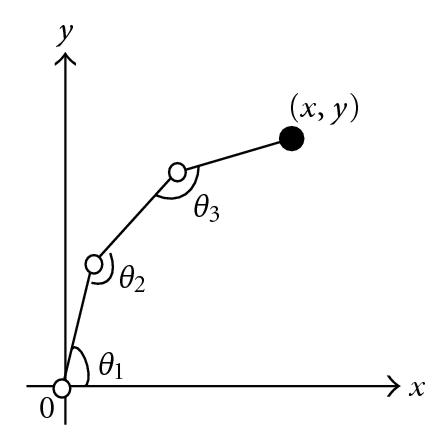
\includegraphics[scale=1.5]{./img/arm_angles.jpg}}
\end{figure}

En cuanto a la función de fitness que se empleará para saber si una solución es buena o no, esta tendra en cuenta el error que comente el soldador en un simulador, segun como de dispersos y desviados sean con respecto al centro dará un valor mayor cuanto peor lo haga y menor cuanto mas preciso sea. Por lo que el objetivo del problemas es minimizar la función de fitness.

Para conocer el error para cada una se las soluciones se hará una llamada get a un servicio que se encuentra en un servidor de la universidad, \href{http://memento.evannai.inf.uc3m.es/age/robot4?}{http://memento.evannai.inf.uc3m.es/age/robot4?}, seguido de cX=GradosDeX para cada uno de los 4 motores y separados por un $\&$, en el caso de los 10 motores será igual, aunque con otro servicio \href{http://memento.evannai.inf.uc3m.es/age/robot10?}{http://memento.evannai.inf.uc3m.es/age/robot10?} y 10 valores de grados.

\section{Programación Estrategia Evolutiva (1+1)}
Para este proyecto entre las posibles implementaciones de las estrategias evolutivas se ha elegido la (1+1)-EE y acontinuación se describiran las caracteristicas de la misma. 

El programa se ha desarrollado en el lenguaje Python, el procesamienot principal del programado se encuentra en la función \textit{EE1plus1(c, cycles, test\_iteration)}, donde recibira como parametros el valor por el que se multiplicaran las varianas, el numero de generaciones maximas del programa y la iteración en la que se encuentra el programa (se incluye para realizar las pruebas de ejecutar multiples veces).

El proceso que sigue esta función es el siguiente:
\begin{enumerate}
	\item Generar el individuo inicial.
	\item Evaluar el individuo generado de la población inicial.
	\item Repetir hasta cumplir el criterio de convergencia:
	\begin{enumerate}
		\item Generar una nueva solución a partir del unico individuo de la población, mutando el vector de codificación del descendiente.
		\item Evaluar el individuo generado.
		\item Eliminar el individuo cuyo valor de adecuación sea mayor, tratamos de minimizar el fitness.
		\item Si el individuo que queda es el nuevo, se aumenta la frecuencia de éxitos y si no se disminuye.
		\item Mutar el vector de varianzas del individuo elegido de acuerdo con la regla 1/5.
	\end{enumerate}
\end{enumerate}

Además de lo relacionado con la generación de individuos, también se ha incluido codigo que nos permita almacenar la salido de los modelos para poderlos evaluar.

\subsection{Operadores genéticos}
\subsubsection{Población inicial}
El individuo inicial es generado aleatoriamente, su vector de codificación siguiendo una gaussiana centrada en 0 y con desviación 100, de esta manera los valores seran tanto positivos como negativos y mayoritariamente centrado en 0, por otro lado el vector de varianzas se genera mediante valores reales positivos entre 5 y 20, aunque se realizaran pruebas con valores mayores.

Este proceso es realizado por la función \textit{initial\_individual()}, devolviendo un individuo en forma de matriz NumeroDeMotores x 2.  

\subsubsection{Mutación}
Para los algoritmos evolutivos este operador se realiza en dos partes una para el vector de codificación y otra para el de varianzas.

Para el vector de codificación, el nuevo individuo tendra como valores los del progenitor mas un valor de la normal segun la varianza de ese valor para el padre, es decir $x_s=x_p+N_0(\sigma_p)$, esta operación se repite para todos los valores del vector.

En cuanto al vector de varianzas, se realizara sobre el individuo seleccionado para la siguietne generación, y consiste en modificar sus varianzas en función de la regla 1/5, que se guia por el porcentaje de mejoras de las ultimas generaciones. Esta regla se aplicara teniendo en cuenta las 10 ultimas generaciones, las variacione vendran dadas por:
\begin{itemize}
	\item Si el numero de mejoras es superior al 20 \%, se aumenta la varianza $\frac \sigma c$.
	\item Si el numero de mejoras es inferior al 20 \%, se reduce la varianza $\sigma \cdot c$.
	\item Si el numero de mejoras es igual al 20 \%, se mantiene $\sigma$.
\end{itemize}

Lo que dice la regla es que si mejora con frecuencia es que todavia estamos lejos de la solución optima y si no mejoramos es que estamos cerca y nos moveremos poco a poco.

Esta funcionalidad se encuentra en la función \textit{mutate\_codification(individual)} para el vector de codificación, aplica la operación para codificación y devuelve al sucesor, y en \textit{individual\_next\_generation(individual, son, improvements\_counter, iteration, c)} para el vector de codificación, se encuentran separadas por que hasta que no se conoce el individuo de la siguiente generación no se muta.

\subsubsection{Inserción y Remplazo}
Al tratarse del tipo (1+1) la población está formada por un solo individuo y también habra un solo individuo, por lo que entre el individuo de la población y el nuevo se elegirá el mejor, en este caso el de menor fitness.

Cuando se elija al descendiente se considera una mejora y se tendra en cuanta en la frecuencia de mejoras, sino se considerar que no ha mejorado. Tras elegir el individuo que formará la población se mutará su vector de varianzas como se a elegido antes.

La función que recoge la inserción y remplazo, ademas de la mutación de las varianzas es la que se mencióno antes, \textit{individual\_next\_generation(individual, son, improvements\_counter, iteration, c)}, que evalua ambos individuos, elige el mejor, actualiza el contador de mejoras y aplica la mutación en función del parametro c que se le pasa. La función devuelve el invididuo elegido, su fitness y el contador de mejoras actualizado. 

\subsection{Aproximación 4 motores}

\begin{figure}[H]
	\ffigbox[\FBwidth]
	{\caption{Valores de Fitness: 4\_5-20\_10}}
	{\includegraphics[scale=.6]{./img/Fitness\_4\_5-20\_10.png}}
\end{figure}
\begin{figure}[H]
	\ffigbox[\FBwidth]
	{\caption{Valores de Fitness: 4\_5-20\_100}}
	{\includegraphics[scale=.58]{./img/Fitness\_4\_5-20\_100.png}}
\end{figure}

\begin{figure}[H]
	\ffigbox[\FBwidth]
	{\caption{Mejores ciclos: 4\_5-20\_10}}
	{\includegraphics[scale=.58]{./img/Cycles\_4\_5-20\_10.png}}
\end{figure}
\begin{figure}[H]
	\ffigbox[\FBwidth]
	{\caption{Mejores ciclos: 4\_5-20\_100}}
	{\includegraphics[scale=.58]{./img/Cycles\_4\_5-20\_100.png}}
\end{figure}

\subsection{Aproximación 10 motores}


\subsection{Resultado}


\section{Conclusiones}


\end{document}